\documentclass{paper}
\usepackage{hyperref}
\usepackage{color}
\usepackage{listings}
\usepackage{graphicx}
\lstset{language=Python,
        stringstyle=\ttfamily,
        escapeinside={*@}{@*}}


\title{TDD of  {\tt Darts}}
\author{Justin Pearson}

\begin{document}
\maketitle
\section{Introduction}
Darts is a game played on a circular board (figure \ref{fig:dartboard}) divided into twenty
numbered  segments. Each segment is divided three areas, single,
double and triple. When a dart hits a segment the score is double or
tripled depending on where it hits.   There is also a bull's eye in
the centre of the board; We will  ignore that.   The players take it in
turns. Each player throws three darts. The score starts at 301 and you
subtract your score from 301. You aim is to get to 0. If you become
negative after throwing your three darts you score is reset to what it
was at the beginning of your round. We assume that every throw scores
something. This is not the official version of darts, but the version
that I used to play in the pub. It will do to illustrate TDD.

\begin{figure}[htb]
  \centering
  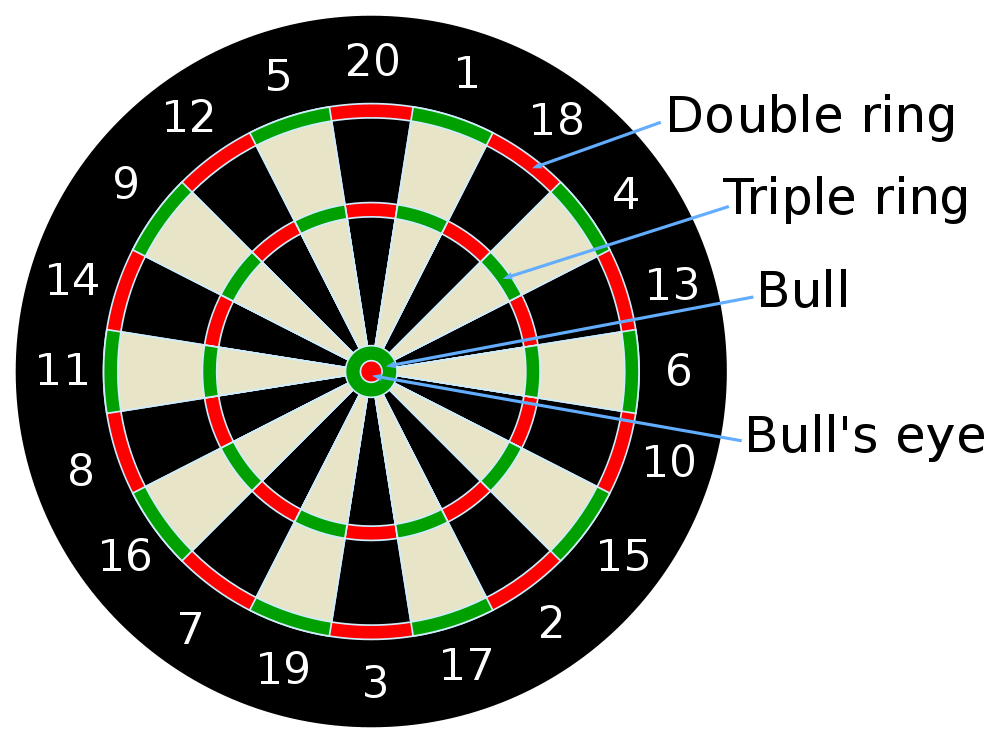
\includegraphics[height=1.86in,width=2.5in]{board.png}
  \caption{A Dart Board}
  \label{fig:dartboard}
\end{figure}
\section{TDD Development of the {\tt scoreboard} class}
We will implement a class that keeps track of the score; which
player's turn it is; and tells us if somebody has won. In a program
this class would probably be interfaced into a GUI. 
\subsection{Red}
So the first test we do is to see if we can initialize an object of
the class.
\begin{lstlisting}
   def test_init(self):
        game  = darts.scoreboard()
\end{lstlisting}
\subsection{Green}
Of course this test will fail. To make the test pass with the minimal
amount of work we do:
\begin{lstlisting}
class scoreboard:
    """ Implements a score board for a darts game """
    pass
\end{lstlisting}
\subsection{Red}
What do we want to do with the class. Darts is a two player game. We
want to know the score of player 1 and the score of player 2.

We assume that we are playing pub darts and start at 301. Games take
to long otherwise, and it takes time away from beer.

\begin{lstlisting}
   def test_score(self):
        game  = darts()
        self.assertEqual(game.playerscore(1),301)
        self.assertEqual(game.playerscore(2),301)
\end{lstlisting}
This fails:
\begin{verbatim}
AttributeError: 'scoreboard' object has no attribute 'playerscore'
\end{verbatim}
\subsection{Green}
So lets make the test pass.
\begin{lstlisting}
class scoreboard:
    """ Implements a score board for a darts game """
    def __init__(self):
        self.playerscores = [301,301]
    def playerscore(self,player):
        return(self.playerscores[player-1])
\end{lstlisting}
\subsection{Red}
We only want two players. We want an exception thrown if we ask for
the score of another player.
\begin{lstlisting}
   def test_exception(self):
        game = darts.scoreboard()
        self.assertRaises(NameError, game.playerscore,3)
\end{lstlisting}
\subsection{Green}
\begin{lstlisting}
      def playerscore(self,player):
        if player == 1 or player == 2:
            return(self.playerscores[player-1])
        else:
            raise NameError('player out of range')

\end{lstlisting}
\subsection{Red}
A dart board is divided into 20 regions. In each region you can score
a single or double or triple times the score. So we want players to
enter their score.
\begin{lstlisting}
      def test_scoring(self):
        game = darts.scoreboard()
        game.playerthrown(1,'single',15)
        self.assertEqual(game.playerscore(1),301-15)
        game.playerthrown(1,'double',20)
        self.assertEqual(game.playerscore(1),301-15-2*20)
        game.playerthrown(1,'triple',5)
        self.assertEqual(game.playerscore(1),301-15-2*20-3*5)
\end{lstlisting}
\subsection{Green}
The test will fail, we do not have a {\tt playerthrown} method. So
first attempt to correct the code:
\begin{lstlisting}
      def playerthrown(player,multiplier,number):
        if multiplier == 'double':
            number = number*2
        elif multiplier == 'triple':
            number = number*3
        self.playerscores[player-1] += number
\end{lstlisting}
Gives the error:
\begin{verbatim}
 TypeError: playerthrown() takes exactly 3 positional arguments (4
 given)
\end{verbatim}
I am still new to Python. I forgot the self argument in the method.
\begin{lstlisting}
      def playerthrown(self,player,multiplier,number):
        if multiplier == 'double':
            number = number*2
        elif multiplier == 'triple':
            number = number*3
        self.playerscores[player-1] += number
\end{lstlisting}
At least it runs, but I still fail the test.
\begin{verbatim}
 self.assertEqual(game.playerscore(1),301-15)
   AssertionError: 316 != 286
\end{verbatim}
Did I get the code wrong or the tests wrong. The test looks fine, but
I want to isolate things so that I can pinpoint the problem.
\begin{lstlisting}
    def test_scoring_single(self):
        game = darts.scoreboard()
        game.playerthrown(1,'single',15)
        self.assertEqual(game.playerscore(1),301-15)
    def test_scoring_double(self):
        game = darts.scoreboard()
        game.playerthrown(1,'double',20)
        self.assertEqual(game.playerscore(1),301-(2*20))
    def test_scoring_triple(self):
        game = darts.scoreboard()
        game.playerthrown(1,'triple',5)
        self.assertEqual(game.playerscore(1),301-(3*5))
\end{lstlisting}
All three tests fail.
\begin{verbatim}
======================================================================
FAIL: test_scoring_double (__main__.TestDarts)
----------------------------------------------------------------------
Traceback (most recent call last):
  File "/var/folders/Ga/Ga5q0tQzEbSDc7-PDs0xgU+++TM/-Tmp-/Python3.21881SBH.py", line 24, in test_scoring_double
    self.assertEqual(game.playerscore(1),301-(2*20))
AssertionError: 341 != 261

======================================================================
FAIL: test_scoring_single (__main__.TestDarts)
----------------------------------------------------------------------
Traceback (most recent call last):
  File "/var/folders/Ga/Ga5q0tQzEbSDc7-PDs0xgU+++TM/-Tmp-/Python3.21881SBH.py", line 20, in test_scoring_single
    self.assertEqual(game.playerscore(1),301-15)
AssertionError: 316 != 286

======================================================================
FAIL: test_scoring_triple (__main__.TestDarts)
----------------------------------------------------------------------
Traceback (most recent call last):
  File "/var/folders/Ga/Ga5q0tQzEbSDc7-PDs0xgU+++TM/-Tmp-/Python3.21881SBH.py", line 28, in test_scoring_triple
    self.assertEqual(game.playerscore(1),301-(3*5))
AssertionError: 316 != 286
\end{verbatim}
Looking at the code, I have made a stupid error.
\begin{lstlisting}
       self.playerscores[player-1] += number
\end{lstlisting}
should be
\begin{lstlisting}
       self.playerscores[player-1] -= number
\end{lstlisting}
Now finally all the test pass.
\subsection{Red}

Darts is a two player game. First player 1 plays 3 shots then player
two plays three shots. We have to decide how the object behaves if
players play out of turn. We will throw exceptions. There are other ways
of doing this, but {\em now} is the time to decide. Write the tests to
capture the behaviour that you want. If you want to change the
behaviour later you will have to rewrite the tests.

\begin{lstlisting}
def test_player_1_plays_first(self):
        game = darts.scoreboard()
        #If a player 2 plays before player 1 then raise an exception.
        self.assertRaises(NameError, game.playerthrown,2,'single',5)   
\end{lstlisting}
Of course the test fails.
\subsection{Green}
 To solve this problem we need a variable that keeps track of the
 state of who's turn it is. So we modify the {\tt init} method.
 \begin{lstlisting}
    def __init__(self):
        self.playerscores = [301,301]
        self.turn = 1
 \end{lstlisting}
And, modify the {\tt playerthrown} method. 
\begin{lstlisting}
      def playerthrown(self,player,multiplier,number):
        if player != turn:
            raise NameError('throw out of turn')
        .....
\end{lstlisting}

Tests still fail. 
\begin{verbatim}
  NameError: global name 'turn' is not defined
\end{verbatim}
I forgot to use {\tt self.turn} instead of {\tt turn}. When it is
fixed all the tests pass.

\subsection{Red}
 Now we have to think about how the game works. 
 You make 3 throws and then it is the other players turn.

 Since we are using exceptions we expect the following code to be
 exception free.

\begin{lstlisting}
  def test_three_throws(self):
       game = darts.scoreboard()
       game.playerthrown(1,'triple',5)
       game.playerthrown(1,'triple',5)
       game.playerthrown(1,'triple',5)
       game.playerthrown(2,'triple',20)
\end{lstlisting}
When the tests run we get an exception when player two tries to throw
a dart.
\subsection{Green}
So we need to keep track of how many throws have been. If we get to 3
then it is the other players turn.

First modify {\tt init}
\begin{lstlisting}
   def __init__(self):
        self.playerscores = [301,301]
        self.turn = 1
        self.throws = 0
\end{lstlisting}
And, then  modify playerthrown to keep track of how many throws and flip the
player when there have been 3 throws.
\begin{lstlisting}
    def playerthrown(self,player,multiplier,number):
        if player != self.turn:
            raise NameError('throw out of turn')
        self.throws = self.throws + 1
        if (self.throws == 3):
            self.turn = 1 - self.turn
\end{lstlisting}
But, the tests still fail.
\begin{verbatim}
======================================================================
ERROR: test_three_throws (__main__.TestDarts)
----------------------------------------------------------------------
Traceback (most recent call last):
  File "/var/folders/rE/rEvVYKXVEFWAJ9IyyNGDqk++42I/-Tmp-/Python3.274950pHt.py", line 38, in test_three_throws
  File "darts.py", line 14, in playerthrown
    raise NameError('throw out of turn')
NameError: throw out of turn

----------------------------------------------------------------------
\end{verbatim}
Ah, I'm stupid. I have a problem with indexing players both by 1 and
by 0. This is going cause more errors in the future. From now on I
will always index the players by 1. So I'll use the trick of having a
dummy entry in the playerscores for the index 0 and rewrite the rest
of the code accordingly. You can't use the turn= 1-turn trick. But at
least the code is easier to write and maintain and understand.
\begin{lstlisting}
  class scoreboard:
    """ Implements a score board for a darts game
    """
    def __init__(self):
        self.playerscores = [None,301,301]
        #  turn = 1 or 2 player's turn.    
        self.turn = 1
        self.throws = 0
    def playerscore(self,player):
        if player == 1 or player == 2:
            return(self.playerscores[player])
        else:
            raise NameError('player out of range')
    def playerthrown(self,player,multiplier,number):
        if player != self.turn:
            raise NameError('throw out of turn')
        self.throws = self.throws + 1
        if (self.throws == 3):
            if (self.turn == 1):
                self.turn = 2
            else:
                self.turn = 1
        if multiplier == 'double':
              number = number*2
        elif multiplier == 'triple':
            number = number*3
        self.playerscores[player] -= number
\end{lstlisting}
Now all the tests pass.

\subsection{Red}
Lets extend the previous test to make sure that we have got the logic
of turns and throws correct.
\begin{lstlisting}
      def test_three_throws(self):
        game = darts.scoreboard()
        game.playerthrown(1,'triple',5)
        game.playerthrown(1,'triple',5)
        game.playerthrown(1,'triple',5)
        game.playerthrown(2,'triple',20)
        game.playerthrown(2,'triple',20)
        game.playerthrown(2,'triple',20)
        game.playerthrown(1,'triple',20)
        self.assertEqual(game.playerscore(1),301-3*(3*5) - 3*20)
        self.assertEqual(game.playerscore(2),301-3*20)
\end{lstlisting}

So we get the error
\begin{verbatim}
======================================================================
ERROR: test_three_throws (__main__.TestDarts)
----------------------------------------------------------------------
Traceback (most recent call last):
  File "/var/folders/rE/rEvVYKXVEFWAJ9IyyNGDqk++42I/-Tmp-/Python3.2749502Yn.py", line 41, in test_three_throws
  File "darts.py", line 16, in playerthrown
    raise NameError('throw out of turn')
NameError: throw out of turn
\end{verbatim}

I'm not sure what is causing the error. So I'll regroup my
tests. It was a bad idea to combine too many tests in one.

\begin{lstlisting}
      def test_player_1_plays_first(self):
        game = darts.scoreboard()
        #If a player 2 plays before player 1 then raise an 
        self.assertRaises(NameError, game.playerthrown,2,'single',5)
    def test_three_throws_1(self):
        game = darts.scoreboard()
        game.playerthrown(1,'triple',5)
        game.playerthrown(1,'triple',5)
        game.playerthrown(1,'triple',5)
        game.playerthrown(2,'triple',20)
    def test_three_throws_2(self):
        game = darts.scoreboard()
        game.playerthrown(1,'triple',5)
        game.playerthrown(1,'triple',5)
        game.playerthrown(1,'triple',5)
        game.playerthrown(2,'triple',20)
        game.playerthrown(2,'triple',20)
        game.playerthrown(2,'triple',20)
    def test_three_throws_3(self):
        game = darts.scoreboard()
        game.playerthrown(1,'triple',5)
        game.playerthrown(1,'triple',5)
        game.playerthrown(1,'triple',5)
        game.playerthrown(2,'triple',20)
        game.playerthrown(2,'triple',20)
        game.playerthrown(2,'triple',20)
        game.playerthrown(1,'triple',20)
        self.assertEqual(game.playerscore(1),301-3*(3*5) - 3*20)
        self.assertEqual(game.playerscore(2),301-3*20)
\end{lstlisting}
\subsection{Green}
The first two tests pass. It is the third that fails. Looking at the
code, I've forgotten to reset the number of throws.
\begin{lstlisting}
     def playerthrown(self,player,multiplier,number):
        if player != self.turn:
            raise NameError('throw out of turn')
        self.throws = self.throws + 1
        if (self.throws == 3):
            self.throws = 0
            if (self.turn == 1):
                self.turn = 2
            else:
                self.turn = 1
        if multiplier == 'double':
              number = number*2
        elif multiplier == 'triple':
            number = number*3
        self.playerscores[player] -= number
\end{lstlisting}
Well the last test still fails.
\begin{verbatim}
  File "/var/folders/rE/rEvVYKXVEFWAJ9IyyNGDqk++42I/-Tmp-/Python3.274950C3C.py", line 57, in test_three_throws_3
AssertionError: 121 != 241
\end{verbatim}
Is it the code or the test? I've miscalculated the score.
This test is getting a bit complicated. We've tested the scoring
system for  player 1. So lets divide the test up a bit.

\begin{lstlisting}
     def test_three_throws_3(self):
        game = darts.scoreboard()
        game.playerthrown(1,'double',5)
        game.playerthrown(1,'double',5)
        game.playerthrown(1,'double',5)
        game.playerthrown(2,'triple',20)
        game.playerthrown(2,'triple',20)
        game.playerthrown(2,'triple',20)
        self.assertEqual(game.playerscore(2),301-3*20)
\end{lstlisting}

This test still fails.
\begin{verbatim}
======================================================================
FAIL: test_three_throws_3 (__main__.TestDarts)
----------------------------------------------------------------------
Traceback (most recent call last):
  File "/var/folders/rE/rEvVYKXVEFWAJ9IyyNGDqk++42I/-Tmp-/Python3.274950Q0n.py", line 55, in test_three_throws_3
AssertionError: 121 != 241
\end{verbatim}
Why do we get the answer 121? Because it is the right answer. I got
the test wrong.
\begin{lstlisting}
    def test_three_throws_3(self):
        game = darts.scoreboard()
        game.playerthrown(1,'double',5)
        game.playerthrown(1,'double',5)
        game.playerthrown(1,'double',5)
        game.playerthrown(2,'triple',20)
        game.playerthrown(2,'triple',20)
        game.playerthrown(2,'triple',20)
        self.assertEqual(game.playerscore(2),301-3*3*20)
\end{lstlisting}
\subsection{Red}
Now lets make the test more complicated. Lets see if we can find a
test to make the code break.
\begin{lstlisting}
      def test_three_throws_4(self):
        game = darts.scoreboard()
        game.playerthrown(1,'double',5)
        game.playerthrown(1,'double',5)
        game.playerthrown(1,'double',5)
        game.playerthrown(2,'triple',20)
        game.playerthrown(2,'triple',20)
        game.playerthrown(2,'triple',20)
        self.assertEqual(game.playerscore(2),301-3*3*20)
        self.assertEqual(game.playerscore(1),301-3*2*5)
        
    def test_three_throws_5(self):
        game = darts.scoreboard()
        game.playerthrown(1,'double',5)
        game.playerthrown(1,'double',5)
        game.playerthrown(1,'double',5)
        game.playerthrown(2,'triple',20)
        game.playerthrown(2,'triple',20)
        game.playerthrown(2,'triple',20)
        self.assertEqual(game.playerscore(2),301-3*3*20)
        self.assertEqual(game.playerscore(1),301-3*2*5)        
        game.playerthrown(1,'single',18)
        self.assertEqual(game.playerscore(1),301-3*2*5-18)
\end{lstlisting}
Well I'm confident that the scoring code works and the players turn
works. You have to stare at the code and think. TDD means you only
have to think about little things at a time. Remember that passing a
bunch of tests does not mean that your code is bug free, you have to
think if you can move on.

What happens when you finish a game of darts. The are variations in
rule sets, but the version I played in the pub is that you must finish
on exactly 0.  Also you must score every throw. I'm not sure what the
real rules are. Anyway this is a quick way for player 1 to get to 0.

\begin{lstlisting}
      def test_win(self):
        # Test what happens when we get to zero.
        game = darts.scoreboard()
        game.playerthrown(1,'triple',20)
        game.playerthrown(1,'triple',20)
        game.playerthrown(1,'triple',20)
        game.playerthrown(2,'single',1)
        game.playerthrown(2,'single',1)
        game.playerthrown(2,'single',1)
        game.playerthrown(1,'double',19)
        game.playerthrown(1,'double',19)
        game.playerthrown(1,'double',19)
        game.playerthrown(2,'single',1)
        game.playerthrown(2,'single',1)
        game.playerthrown(2,'single',1)
        game.playerthrown(1,'single',1)
        game.playerthrown(1,'single',3)
        game.playerthrown(1,'single',3)
        self.assertEqual(game.playerscore(1),0)
\end{lstlisting}
Well we still have not reached condition red. This test passes. We
have to decide what we want the class to do when a player wins. 
The alternatives are  Exceptions, or  Special value for the score?

Personally I like using exceptions for non-error conditions, but some
people think this is a bad idea. In some languages exceptions also
have unnecessary extra overhead. So since this scoreboard will
probably be interfaced to a GUI, we'll return a string 'WON' when the
score goes to 0.

So lets modify the last line of the test.
        self.assertEqual(game.playerscore(1),'WON')
The test fails. 

\subsection{Green}
 So lets make the score function return 'WON' if the score is 0.
 \begin{lstlisting}
       def playerscore(self,player):
        if player == 1 or player == 2:
            if (self.playerscores[player] != 0 ): 
                return(self.playerscores[player])
            else:
                return('WON')
        else:
            raise NameError('player out of range')
 \end{lstlisting}
All tests pass.
\subsection{Red}
If you get a negative score during a throw then your score is reset
back to what it was before the throw (in some variants you have to end
on a double as well, we won't bother with that).  So we can modify the
previous test.
\begin{lstlisting}
      def test_win_2(self):
        # Test what happens when we get to zero.
        game = darts.scoreboard()
        game.playerthrown(1,'triple',20)
        game.playerthrown(1,'triple',20)
        game.playerthrown(1,'triple',20)
        game.playerthrown(2,'single',1)
        game.playerthrown(2,'single',1)
        game.playerthrown(2,'single',1)
        game.playerthrown(1,'double',19)
        game.playerthrown(1,'double',19)
        game.playerthrown(1,'double',19)
        game.playerthrown(2,'single',1)
        game.playerthrown(2,'single',1)
        game.playerthrown(2,'single',1)
        game.playerthrown(1,'single',1)
        game.playerthrown(1,'single',3)
        game.playerthrown(1,'triple',20)
        self.assertNotEqual(game.playerscore(1),'WON')
        game.playerthrown(2,'single',1)
        game.playerthrown(2,'single',1)
        game.playerthrown(2,'single',1)
        game.playerthrown(1,'single',1)
        game.playerthrown(1,'single',3)
        game.playerthrown(1,'single',3)
        self.assertEqual(game.playerscore(1),'WON')
\end{lstlisting}
You really should refactor the test cases. I'll leave these to
you. When you run the tests you get:
\begin{verbatim}
Traceback (most recent call last):
  File "/var/folders/rE/rEvVYKXVEFWAJ9IyyNGDqk++42I/-Tmp-/Python3.2749503Zu.py", line 126, in test_win_2
AssertionError: -64 != 'WON'
\end{verbatim}
So we'll need to keep track of the score in the current round.
Modify {\tt init}.
\begin{lstlisting}
   def __init__(self):
        self.playerscores = [None,301,301]
        #  turn = 1 or 2 player's turn.    
        self.turn = 1
        self.throws = 0
        self.current_round = 0
\end{lstlisting}
When we flip the current player we'll check if the score is -ve. If it
is then we'll add the {\tt current\_round} score back to the score so the
score should be reset to the score before the round.

\begin{lstlisting}
  def playerthrown(self,player,multiplier,number):
        if player != self.turn:
            raise NameError('throw out of turn')
        self.throws = self.throws + 1
        if (self.throws == 3):
            self.throws = 0
            if self.playerscores[player] < 0:
                self.playerscores[player] += self.current_round                
            self.current_round = 0
            if (self.turn == 1):
                self.turn = 2
            else:
                self.turn = 1
        if multiplier == 'double':
              number = number*2
        elif multiplier == 'triple':
            number = number*3
        self.playerscores[player] -= number
        self.current_round += number
\end{lstlisting}
The code still does not pass all the tests.
\begin{verbatim}
FAIL: test_win_2 (__main__.TestDarts)
----------------------------------------------------------------------
Traceback (most recent call last):
  File "/var/folders/rE/rEvVYKXVEFWAJ9IyyNGDqk++42I/-Tmp-/Python3.274950D4J.py", line 126, in test_win_2
AssertionError: -59 != 'WON'

----------------------------------------------------------------------
\end{verbatim}
Let's make the test a little more fine grained.
\begin{lstlisting}
   def test_win_2(self):
        # Test what happens when we get to zero.
        game = darts.scoreboard()
        game.playerthrown(1,'triple',20)
        game.playerthrown(1,'triple',20)
        game.playerthrown(1,'triple',20)
        game.playerthrown(2,'single',1)
        game.playerthrown(2,'single',1)
        game.playerthrown(2,'single',1)
        game.playerthrown(1,'double',19)
        game.playerthrown(1,'double',19)
        game.playerthrown(1,'double',19)
        current_score_player_1 = game.playerscore(1)
        game.playerthrown(2,'single',1)
        game.playerthrown(2,'single',1)
        game.playerthrown(2,'single',1)
        game.playerthrown(1,'single',1)
        game.playerthrown(1,'single',3)
        game.playerthrown(1,'triple',20)
        self.assertEqual(game.playerscore(1),current_score_player_1)
        self.assertNotEqual(game.playerscore(1),'WON')
        game.playerthrown(2,'single',1)
        game.playerthrown(2,'single',1)
        game.playerthrown(2,'single',1)
        game.playerthrown(1,'single',1)
        game.playerthrown(1,'single',3)
        game.playerthrown(1,'single',3)
        self.assertEqual(game.playerscore(1),'WON')
\end{lstlisting}
It still fails.
\begin{verbatim}
======================================================================
FAIL: test_win_2 (__main__.TestDarts)
----------------------------------------------------------------------
Traceback (most recent call last):
  File "/var/folders/rE/rEvVYKXVEFWAJ9IyyNGDqk++42I/-Tmp-/Python3.274950R1u.py", line 120, in test_win_2
    self.assertEqual(game.playerscore(1),current_score_player_1)
AssertionError: -57 != 7

----------------------------------------------------------------------
\end{verbatim}
So I must of got the logic wrong for incrementing and decrementing the
score. I got the current round logic wrong. Before when I flipped it
did not affect the rest of the code. Now I have to flip in the right place.
I cheated I added print statements to see what was going wrong. Old
habits die hard!

New code.
\begin{lstlisting}
      def playerthrown(self,player,multiplier,number):
        #Check if it the right players turn.
        if player != self.turn:
            raise NameError('throw out of turn')
        #Now it is safe to increment the number of throws.
        self.throws = self.throws + 1
        #If we've down 3 throws then it is somebody else's turn.

        #Now work out the score.
        if multiplier == 'double':
              number = number*2
        elif multiplier == 'triple':
            number = number*3
        #Change the current score.
        self.playerscores[player] -= number
        self.current_round += number
        #If we have done 3 throws then
        # 1) we need to flip
        # 2) we need to our score is -ve.
        # 3) We need to reset the current_score to 0.
        if (self.throws == 3):
            self.throws = 0
            #This if statement flips the players turn.
            if (self.turn == 1):
                self.turn = 2
            else:
                self.turn = 1
            #Now we check if our score is -ve
            if self.playerscores[player] < 0:
                self.playerscores[player] += self.current_round
            #Now reset the current_round
            self.current_round = 0
        #That's the end of the 3 throws logic.
\end{lstlisting}
All tests are passed. The code is working. 
The method is kind of long. There is plenty of scope to refactor the
code. 

\section{Complete Test Code}
\begin{lstlisting}
import darts
import unittest


class TestDarts(unittest.TestCase):
    def test_init(self):
        game  = darts.scoreboard()
    def test_score(self):
        game  = darts.scoreboard()
        self.assertEqual(game.playerscore(1),301)
        self.assertEqual(game.playerscore(2),301)
    def test_exception(self):
        game = darts.scoreboard()
        self.assertRaises(NameError, game.playerscore,3)
    def test_scoring_single(self):
        game = darts.scoreboard()
        game.playerthrown(1,'single',15)
        self.assertEqual(game.playerscore(1),301-15)
    def test_scoring_double(self):
        game = darts.scoreboard()
        game.playerthrown(1,'double',20)
        self.assertEqual(game.playerscore(1),301-(2*20))
    def test_scoring_triple(self):
        game = darts.scoreboard()
        game.playerthrown(1,'triple',5)
        self.assertEqual(game.playerscore(1),301-(3*5))
    def test_player_1_plays_first(self):
        game = darts.scoreboard()
        #If a player 2 plays before player 1 then raise an 
        self.assertRaises(NameError, game.playerthrown,2,'single',5)
    def test_three_throws_1(self):
        game = darts.scoreboard()
        game.playerthrown(1,'triple',5)
        game.playerthrown(1,'triple',5)
        game.playerthrown(1,'triple',5)
        game.playerthrown(2,'triple',20)
    def test_three_throws_2(self):
        game = darts.scoreboard()
        game.playerthrown(1,'triple',5)
        game.playerthrown(1,'triple',5)
        game.playerthrown(1,'triple',5)
        game.playerthrown(2,'triple',20)
        game.playerthrown(2,'triple',20)
        game.playerthrown(2,'triple',20)
    def test_three_throws_3(self):
        game = darts.scoreboard()
        game.playerthrown(1,'double',5)
        game.playerthrown(1,'double',5)
        game.playerthrown(1,'double',5)
        game.playerthrown(2,'triple',20)
        game.playerthrown(2,'triple',20)
        game.playerthrown(2,'triple',20)
        self.assertEqual(game.playerscore(2),301-3*3*20)

    def test_three_throws_4(self):
        game = darts.scoreboard()
        game.playerthrown(1,'double',5)
        game.playerthrown(1,'double',5)
        game.playerthrown(1,'double',5)
        game.playerthrown(2,'triple',20)
        game.playerthrown(2,'triple',20)
        game.playerthrown(2,'triple',20)
        self.assertEqual(game.playerscore(2),301-3*3*20)
        self.assertEqual(game.playerscore(1),301-3*2*5)
        
    def test_three_throws_5(self):
        game = darts.scoreboard()
        game.playerthrown(1,'double',5)
        game.playerthrown(1,'double',5)
        game.playerthrown(1,'double',5)
        game.playerthrown(2,'triple',20)
        game.playerthrown(2,'triple',20)
        game.playerthrown(2,'triple',20)
        self.assertEqual(game.playerscore(2),301-3*3*20)
        self.assertEqual(game.playerscore(1),301-3*2*5)        
        game.playerthrown(1,'single',18)
        self.assertEqual(game.playerscore(1),301-3*2*5-18)

    def test_win_1(self):
        # Test what happens when we get to zero.
        game = darts.scoreboard()
        game.playerthrown(1,'triple',20)
        game.playerthrown(1,'triple',20)
        game.playerthrown(1,'triple',20)
        game.playerthrown(2,'single',1)
        game.playerthrown(2,'single',1)
        game.playerthrown(2,'single',1)
        game.playerthrown(1,'double',19)
        game.playerthrown(1,'double',19)
        game.playerthrown(1,'double',19)
        game.playerthrown(2,'single',1)
        game.playerthrown(2,'single',1)
        game.playerthrown(2,'single',1)
        game.playerthrown(1,'single',1)
        game.playerthrown(1,'single',3)
        game.playerthrown(1,'single',3)
        self.assertEqual(game.playerscore(1),'WON')
        
    def test_win_2(self):
        # Test what happens when we get to zero.
        game = darts.scoreboard()
        game.playerthrown(1,'triple',20)
        game.playerthrown(1,'triple',20)
        game.playerthrown(1,'triple',20)
        game.playerthrown(2,'single',1)
        game.playerthrown(2,'single',1)
        game.playerthrown(2,'single',1)
        game.playerthrown(1,'double',19)
        game.playerthrown(1,'double',19)
        game.playerthrown(1,'double',19)
        current_score_player_1 = game.playerscore(1)
        game.playerthrown(2,'single',1)
        game.playerthrown(2,'single',1)
        game.playerthrown(2,'single',1)
        game.playerthrown(1,'single',1)
        game.playerthrown(1,'single',3)
        game.playerthrown(1,'triple',20)
        self.assertEqual(game.playerscore(1),current_score_player_1)
        self.assertNotEqual(game.playerscore(1),'WON')
        game.playerthrown(2,'single',1)
        game.playerthrown(2,'single',1)
        game.playerthrown(2,'single',1)
        game.playerthrown(1,'single',1)
        game.playerthrown(1,'single',3)
        game.playerthrown(1,'single',3)
        self.assertEqual(game.playerscore(1),'WON')

        
if __name__ == '__main__':
    unittest.main()
\end{lstlisting}
\section{Final implementation}
\begin{lstlisting}
class scoreboard:
    """ Implements a score board for a darts game
    """
    def __init__(self):
        self.playerscores = [None,301,301]
        #  turn = 1 or 2 player's turn.    
        self.turn = 1
        self.throws = 0
        self.current_round = 0
    def playerscore(self,player):
        if player == 1 or player == 2:
            if (self.playerscores[player] != 0 ): 
                return(self.playerscores[player])
            else:
                return('WON')
        else:
            raise NameError('player out of range')

    def playerthrown(self,player,multiplier,number):
        #Check if it the right players turn.
        if player != self.turn:
            raise NameError('throw out of turn')
        #Now it is safe to increment the number of throws.
        self.throws = self.throws + 1
        #If we've down 3 throws then it is somebody else's turn.

        #Now work out the score.
        if multiplier == 'double':
              number = number*2
        elif multiplier == 'triple':
            number = number*3
        #Change the current score.
        self.playerscores[player] -= number
        self.current_round += number
        #If we have done 3 throws then
        # 1) we need to flip
        # 2) we need to our score is -ve.
        # 3) We need to reset the current_score to 0.
        if (self.throws == 3):
            self.throws = 0
            #This if statement flips the players turn.
            if (self.turn == 1):
                self.turn = 2
            else:
                self.turn = 1
            #Now we check if our score is -ve
            if self.playerscores[player] < 0:
                self.playerscores[player] += self.current_round
            #Now reset the current_round
            self.current_round = 0
        #That's the end of the 3 throws logic.


    


\end{lstlisting}
\end{document}

